%% Default Latex document template
%%
%%  blake@rcs.ee.washington.edu

\documentclass[letterpaper]{article}

% Uncomment for bibliog.
%\bibliographystyle{unsrt}

\usepackage{graphicx}
% \usepackage{lineno}
%\usepackage{fancyhdr}

%%%%%%%%%%%%%%%%%%%%%%%%%%%%%%%%%%%%%%%%5
%
%  Set Up Margins

%%%%%%%%%%%%%%%%%%%%%%%%%%%%%%%%%%%%%%%%%%%%%%%%%
% include file for:
%      Critical Page setup dimensions
%            DO NOT MODIFY
%       (for help see "Latex Line by Line" p 260)
%
\setlength\oddsidemargin{0in}
\setlength\evensidemargin{0in}

\usepackage[left=0.98in, right=0.98in, top=1.0in, bottom=1.0in]{geometry}

% %Top Margin and header
% \setlength\voffset{-0.94in}
% \setlength\topmargin{0.25in}
% \setlength\headheight{0.25in}
% %\setlength\headwidth{6.5in}
% \setlength\headsep{0.25in}
% %Body
% \setlength\textwidth{6.5in}
% \setlength\textheight{9.50in}
% %Footer
% %\setlength\footheight{0.5in}
% \setlength\footskip{0.3750in}
% Line spacing for 6 lines per inch
\linespread{0.894}  % 1.0 = single    1.6 = double
%
%          END of Critical Page Setup Dimensions
%%%%%%%%%%%%%%%%%%%%%%%%%%%%%%%%%%%%%%%%%%%%%%%%%%%

%%%%%%%%%%%%%%%%%%%%%%%%%%%%%%%%%%%%%%%%%%%%%%%%%%%
%
% Useful style and math macros
%


\newcommand\Dfrac[2]{\frac{\displaystyle #1}{\displaystyle #2}}
\newcommand\beq{\begin{equation}}
    \newcommand\eeq{\end{equation}}

\newcommand\bmat{\begin{bmatrix}}
    \newcommand\emat{\end{bmatrix}}

\newenvironment{solution}
{\ttfamily \vspace{0.155in} {\bf SOLUTION:} \\ }
{ \vspace{0.25in} \par }


% Make table rows deeper
%\renewcommand\arraystretch{2.0}% Vertical Row size, 1.0 is for standard spacing)


%
%        Font selection
%
%\renewcommand{\rmdefault}{ptm}             % Times
%\renewcommand{\rmdefault}{phv}             % Helvetica
%\renewcommand{\rmdefault}{pcr}             % Courier
%\renewcommand{\rmdefault}{pbk}             % Bookman
%\renewcommand{\rmdefault}{pag}             % Avant Garde
%\renewcommand{\rmdefault}{ppl}             % Palatino
%\renewcommand{\rmdefault}{pch}             % Charter


%%%%%%%%%%%%%%%%%%%%%%%%%%%%%%%%%%%%%%%%%%%%%%%%%
%
%         Page format Mods HERE
%
%Mod's to page size for this document
\addtolength\textwidth{0cm}
\addtolength\oddsidemargin{0cm}
\addtolength\headsep{0cm}
\addtolength\textheight{0cm}
%\linespread{0.894}   % 0.894 = 6 lines per inch, 1 = "single",  1.6 = "double"

%\lhead{LEFT HEADER}
%\chead{CENTER HEADER}
%\rhead{RIGHT HEADER}
%\lfoot{Hannaford, U. of Washington}
%\rfoot{\today}
%\cfoot{\thepage}

% Make table rows deeper
%\renewcommand\arraystretch{2.0}% Vertical Row size, 1.0 is for standard spacing)
\usepackage{tikz}
\usetikzlibrary{calc,patterns,decorations.pathmorphing,decorations.markings,calc}

\usetikzlibrary{circuits}
\usetikzlibrary{circuits.ee.IEC}

\begin{document}
% \setpagewiselinenumbers        %  Line numbers for edits to drafts.
% \modulolinenumbers[1]          %  number every N lines

% \linenumbers                   %  start numbering lines here
% %
%  \node (M) [minimum width=3.5cm,minimum height=2cm] {$m_1$};
% %
% % %  left most spring ground
%  \node (ground1) at (M.south) [ground,yshift=-1.5cm,xshift=-1.25cm,anchor=north] {};
%  \draw (ground1.north west) -- (ground1.north east);
%  \draw [spring] (ground1.north) -- ($(M.south east)!(ground1.north)!(M.south west)$);
% %
%  % damper ground
%  \node (ground2) at (M.south) [ground,yshift=-1.5cm,anchor=north] {};
%  \draw (ground2.north west) -- (ground2.north east);
%  \draw [damper] (ground2.north) -- ($(M.south east)!(ground2.north)!(M.south west)$);
% %
%  % right spring ground
%  \node (ground3) at (M.south) [ground,yshift=-1.5cm,xshift=1.25cm,anchor=north] {};
%  \draw (ground3.north west) -- (ground3.north east);
%  \draw [spring] (ground3.north) -- ($(M.south east)!(ground3.north)!(M.south west)$);
% %
% % % up arrow vector
%  \draw [-latex,ultra thick] (M.north) ++(0,0.2cm) -- +(0,1cm);
% %
% %
% % %%%%%%%%%%%%%%%%%%%%%%%%%%%%%%%%%%%%%%%%%
%  \begin{scope}[xshift=7cm]
%  \node (M) [minimum width=1cm, minimum height=2.5cm] {$m$};
%
%  \node (ground) [ground,anchor=north,yshift=-0.25cm,minimum width=1.5cm] at (M.south) {};
%  \draw (ground.north east) -- (ground.north west);
% %
% % % little wheels
%  \draw [thick] (M.south west) ++ (0.2cm,-0.125cm) circle (0.125cm)  (M.south east) ++ (-0.2cm,-0.125cm) circle (0.125cm);
% %
%  \node (wall) [ground, rotate=-90, minimum width=3cm,yshift=-3cm] {};
%  \draw (wall.north east) -- (wall.north west);
% %
%  \draw [spring] (wall.170) -- ($(M.north west)!(wall.170)!(M.south west)$);
%  \draw [damper] (wall.10) -- ($(M.north west)!(wall.10)!(M.south west)$);
% %
%  \draw [-latex,ultra thick] (M.east) ++ (0.2cm,0) -- +(1cm,0);
%  \end{scope}
%  \end{tikzpicture}
% %
%



%%%%%%%%%%%%%%%%%%%%%%%%%%%%%%%%%%%%%%%%%%%%%%%%%%%%%%%%%%%%%%%%%%%%%%%%%%%%%%%%%%%%%%%%

%        Closed loop control system

%%%%%%%%%%%%%%%%%%%%%%%%%%%%%%%%%%%%%%%%%%%%%%%%%%%%%%%%%%%%%%%%%%%%%%%%%%%%%%%%%%%%%%%%

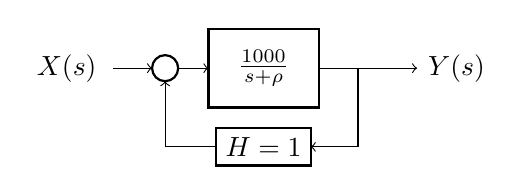
\begin{tikzpicture}[every node/.style={draw, thick,outer sep=0pt,thick}]

% %
% debugging grid
%  \draw[step=5mm,gray,very thin] (-25mm,-25mm) grid (100mm,50mm);
%  \draw[thick,gray] (0,-25mm) -- (0,50mm);
%  \draw[thick,gray] (-25mm,0) -- (100mm,0);
%
%
%

 \node (C) [thick,minimum width=14mm, minimum height=10mm] {$\frac{1000}{s+\rho}$};
 \node (H) [thick, yshift=-10mm] {$H=1$};

 \coordinate (outend) at ($(C.east)+(12.5mm,0)$);
 \coordinate (out2)   at ($(C.east)+(5mm,0)$);
 \draw [->] (C.east) -- (outend);
 \draw [->]  (out2)   -- ++(0,-10mm) -- (H.east);

 \node (sum)   [circle,draw,minimum width=0.1cm ] at (-12.5mm,0mm) {};

 \draw [->] (H.west) -- (-12.5mm,-10mm) -- (sum.south);

 \draw [->] (sum.east) -- (C.west);
 \draw [<-] (sum.west) -- ++(-5mm,0mm);

\tikzstyle{every node}=[];

 \coordinate  (input) at ($(sum.west)+(-5mm,0)$) node[xshift=-25mm] {$X(s)$};

 \node (output) at ($(outend)+(5mm,0mm)$) {$Y(s)$};




% \draw [thick] (Mc.east)  --  (Xa);

\end{tikzpicture}

%  Use name of bibliography files without .bib extension
%\bibliography{brl}
\end{document}

